\documentclass[a4paper,12pt]{article}

\usepackage{amsmath,amssymb,amsthm,multicol,tikz,enumitem}
\usepackage{hyperref}
\usepackage{fancyvrb}
%\usepackage{enumerate}
\usepackage[margin=2cm]{geometry}
\usetikzlibrary{calc,arrows.meta}

\newcommand\N{\mathbf{N}}
\newcommand\Q{\mathbf{Q}}
\newcommand\R{\mathbf{R}}
\newcommand\Z{\mathbf{Z}}

\def\ojoin{\setbox0=\hbox{$\bowtie$}%
  \rule[-.02ex]{.25em}{.4pt}\llap{\rule[\ht0]{.25em}{.4pt}}}
\def\leftouterjoin{\mathbin{\ojoin\mkern-5.8mu\bowtie}}
\def\rightouterjoin{\mathbin{\bowtie\mkern-5.8mu\ojoin}}
\def\fullouterjoin{\mathbin{\ojoin\mkern-5.8mu\bowtie\mkern-5.8mu\ojoin}}

% Comment out one or the other

\ifdefined\mysolution
  \newcommand\answer[1]{\mbox{}\\[-15pt]{\color{blue}{#1}}\hfill{\color{blue}$\qed$}\mbox{}\\[-15pt]} 
  \newcommand\ans[1]{{\color{blue}{#1}}}
\else 
  \newcommand\answer[1]{}
  \newcommand\ans[1]{}
\fi


\setlength{\parindent}{0pt}

\begin{document}

\thispagestyle{empty}

\begin{center}
{\bf\Huge 4.\ mājasdarbs} \\[5pt]
Lietišķie algoritmi, 2019.g.\ rudens\\
Termiņš: 2019-12-09
\end{center}

\hrule
\vspace{2pt}
\hrule
\vspace{12pt}



\vspace{6pt}
{\bf 1.uzdevums: RSA algoritms.} 
Bobs vēlas izveidot savu privātās/publiskās 
atslēgas pāri $(n,e)$, kur $n = p \cdot q$ ir reizinājums diviem 
mazākajiem $17$-ciparu pirmskaitļiem (un $p<q$), bet kā 
publisko kāpinātāju viņš grib izvēlēties skaitli $e = 2^{16} + 1$.
\begin{enumerate}[label=(\alph*)]
\item Kādi ir pirmskaitļi $p$ un $q$ un to reizinājums $n$?
(Lielu pirmskaitļu pārbaudīšanai var izmantot esošas bibliotēkas, kas
implementē Rabina-Millera varbūtisko pirmskaitļu pārbaudi, 
piemēram Python funkciju {\tt sympy.isprime}.)
\item Alise grib nosūtīt ziņojumu $m = 100$, izmantojot 
publisko RSA kriptoatslēgu - pāri $(n,e)$. Kāds ir viņas 
iešifrētais ziņojums?
\item Cik reizināšanas darbības pēc $n$ moduļa Alisei jāveic, lai
iešifrētu $m$?
\item Kāda ir Boba izmantotā privātā kriptoatslēga $d$, kurai 
ir spēkā $e \cdot d \equiv 1$ pēc $\varphi(n)$ moduļa?
\item Cik reizināšanas darbības pēc $n$ moduļa Bobam jāveic, lai 
atšifrētu Alises iešifrēto ziņojumu?
\end{enumerate}

\answer{

{\bf (a)} Mazākais $17$-ciparu skaitlis ir $10^{16}$ (viens vieninieks
un sešpadsmit nulles). Izmantojot nelielu Python programmiņu, 
iegūstam, ka $p=10000000000000061$ un $q=10000000000000069$. To reizinājums
$$n = pq = 100000000000001300000000000004209.$$ 
Sk. attēlu~\ref{fig:python-primes}

\begin{figure}[!htb]
\center{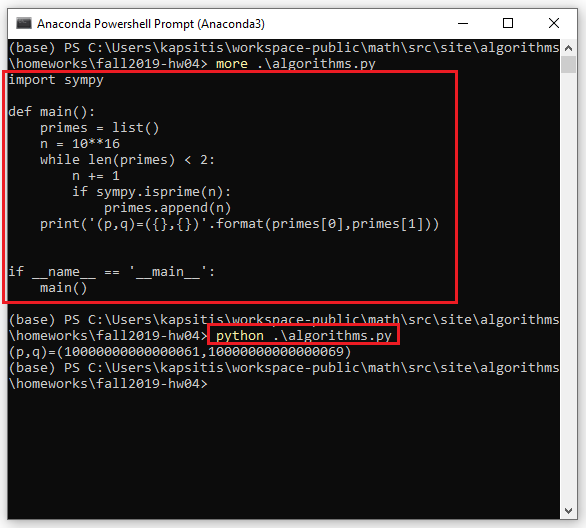
\includegraphics[width=3in]{fall2019-hw04/python-primes.png}}
\caption{\label{fig:python-primes} Pirmskaitļu meklēšana}
\end{figure}



\vspace{6pt}
{\bf (b)} Alise nosūta skaitli $m^e\;(\text{mod}\,n)$. Mūsu gadījumā $m=100$,
$e = 2^{16} + 1$, $n = pq$. Lai kāpinātu pakāpē $e$, izmantojam nevis atkārtotu reizināšanu
ciklā (kas prasītu ļoti daudz laika), bet gan sešpadsmit reizes kāpinām skaitli $m=100$
kvadrātā un pēc tam vēlreiz piereizinām ar $m$. 

Iegūtais kriptoteksts ir šāds:
$$m^e\;(\text{mod}\,n) = 14901635321531082019468095932167.$$

\vspace{6pt}
{\bf (c)} Iepriekš aprakstītajā aprēķinā Alise veica $16+1 = 17$ reizināšanas darbības:
16 reizes reizināja skaitli pašu ar sevi (un atrada atlikumu), pēdējā solī vēlreiz
piereizināja ar $m=100$.

\vspace{6pt}
{\bf (d)} Privāta kriptoatslēga, ko izmanto Bobs ir $d = e^{-1}\;(\text{mod}\,(p-1)(q-1))$.
Šeit $e = 2^{16} + 1$; tātad jāatrod skaitlis $d$, kuru piereizinot ar $e$ iegūsim atlikumu $1$,
dalot ar $(p-1)(q-1)$.
Darbinām citu scenāriju, lai atrastu skaitlim $e = 2^{16}+1$ inverso. Sk., piemēram, 
\url{https://bit.ly/378djaG}.

Iegūstam šādu atslēgas vērtību:
$$d = 93617345926729611259593817236833$$
Atšifrēšanas pareizuma pārbaudei var izmantot Pitona iebūvēto funkciju {\tt pow(x,y,m)}, kas
kāpina $x$ pakāpē $y$ pēc $m$ moduļa:\\


{\tt decrypt = pow(encrypt,d,n)}\\
{\tt print('decrypted = \{\}'.format(decrypt))}\\


{\bf (e)} Iepriekšējā solī atšifrēšana (kāpināšana lielajā pakāpē $d$)
notika ar iebūvētu Pitona funkciju {\tt pow(x,y,m)}. Ja mums pašiem tā
būtu efektīvi jāuzprogrammē,
kāpinātāju $d$ pārveidojam divnieku skaitīšanas sistēmā (var izmantot Pitona
iebūvēto funkciju {\tt bin(...)}.

Iegūtais skaitlis ir (skaitļa pierakstā ir $107$ binārie cipari, no tiem $55$ ir vieninieki).
$$d = (1001001110\ldots{}0101100001)_2.$$
Kāpināšanai šādā pakāpē, izmantojot {\em Exponentiation by Squaring} metodi,
vajag $107-1 = 106$ reizes kāpināt kvadrātā un arī $55-1 = 54$ reizes
piereizināt kāpināmo skaitli. Pavisam tātad $160$ reizināšanas.

{\bf Piezīme.} Ievērosim, ka Alisei, kāpinot pakāpē $e = 2^{16}+1$, vajadzēja tikai $17$
reizināšanas, bet atšifrēšanai jeb kāpināšanai pakāpē $d$ vajag $160$ reizināšanas.
Asimetriskiem algoritmiem 
iešifrēšana un atšifrēšana var būtiski atšķirties laika sarežģītības ziņā. Mūsu gadījumā
publiskā atslēga $e = 2^{16}+1$ tika
izraudzīta tā, lai iešifrēt varētu īpaši ātri.

}




\vspace{6pt}
{\bf 2.uzdevums: Afīnās mērogošanas metode LP uzdevumā.}
Dots LP uzdevums: Maksimizēt $2x_1 + 3x_2$, kur
$$\left\{ \begin{array}{l}
x_1 - 2x_2 \leq 4,\\
x_1 + x_2 \leq 18,\\
x_2 \leq 10,\\
x_1,x_2 \geq 0.
\end{array} \right.$$
Aprēķināt un attēlot koordinātu plaknē šī LP uzdevuma pirmos $2$ tuvinājumus 
$X(1)$ un $X(2)$ kā $2$-dimensionālus vektorus, izmantojot 
afīnās skalēšanas metodi.\\ 
Izvēlētais sākumpunkts $X(0) = (5,5)$ (t.i. sākumpunkta
koordinātes ir $x_1 = 5$ un $x_2 = 5$). Gan $X(1)$, gan $X(2)$ abas koordinātes
atbildē noapaļot līdz $5$ cipariem aiz komata. Soļa garums abos 
gadījumos: $\beta = 0.96$. (Vektoru un matricu operācijām var izmantot Python bibliotēkas.)



\vspace{6pt}
{\bf 3.uzdevums: KMP un BM algoritmi.} 
% https://www.csie.ntu.edu.tw/~hsinmu/courses/_media/dsa_17spring/dsa_2017_hw2_sol_1.pdf
Virknē {\tt 947892879487} meklējam apakšstringu {\tt 9487}.
\begin{enumerate}[label=(\alph*)]
\item Atrast Knuta-Morisa-Prata algoritmam vajadzīgo prefiksu funkciju $\pi$. 
\item Atrast Bojera-Mūra algoritmam vajadzīgo labo sufiksu tabulu un sliktā simbola tabulu.
\end{enumerate}

\answer{

{\bf (a)} Izveidojam tabuliņu prefiksu funkcijai:

\begin{tabular}{|r||c|c|c|c|} \hline
$j$ & 1 & 2 & 3 & 4 \\ \hline
$\pi(j)$ & 0 & 0 & 0 & 0 \\ \hline
\end{tabular}

{\bf (b)} Izveidojam sliktā simbola tabulu \textendash{} atzīmējam tabuliņā pēdējo indeksu,
ar kuru simbols ietilpst paraugā $P = \mathtt{9487}$ vai $-1$, ja simbola tur nav vispār.
Šeit $\mathtt{\ast}$ apzīmē visus citus simbolus, izņemot tabulā ierakstītos.

\begin{tabular}{|r||c|c|c|c|c|} \hline
$x$ & $\mathtt{4}$ & $\mathtt{7}$ & $\mathtt{8}$ & $\mathtt{9}$ & $\mathtt{\ast}$ \\ \hline
$\lambda(x)$ & 1 & 3 & 2 & 0 & -1 \\ \hline
\end{tabular}


}



\vspace{6pt}
{\bf 4.uzdevums: Bojera-Mūra algoritms.}
Dots teksts $T = \mathtt{abcabbcabcbcababababcbcab}$ un meklējamais paraugs
$P = \mathtt{abcbcab}$. 
\begin{enumerate}[label=(\alph*)]
\item Uzrakstīt Bojera-Mūra algoritmā lietotās tabulas apakšstringam $P$.
\item Nodemonstrēt Bojera-Mūra darbību pa soļiem, meklējot paraugu $P$ dotajā tekstā $T$.
\end{enumerate}


\answer{


\vspace{2ex}
{\bf (a)} Sliktā simbola tabula (tikai $3$ burti, jo citu tekstā un paraugā nav):

\begin{tabular}{|r||c|c|c|} \hline
$x$ & {\tt a} & {\tt b} & {\tt c} \\ \hline
$\lambda(x)$ & 5 & 6 & 4 \\ \hline
\end{tabular}

Labā sufiksa tabulu aprēķināsim, vispirms atrodot prefiksu funkcijas $\pi$ 
un $\pi'$ paraugam $P = \mathtt{abcbcab}$ un reversajam paraugam 
$P' = \mathtt{bacbcba}$ (no otra gala uzrakstītam paraugam). 

\begin{tabular}{|r||c|c|c|c|c|c|c|} \hline
$\ell$              & 1 & 2 & 3 & 4 & 5 & 6 & 7 \\ \hline
$\pi(\ell)$         & 0 & 0 & 0 & 0 & 0 & 1 & 2 \\ \hline
$\pi'(\ell)$        & 0 & 0 & 0 & 1 & 0 & 1 & 2 \\ \hline
$\ell - \pi'(\ell)$ & 1 & 2 & 3 & 3 & 5 & 5 & 5 \\ \hline
\end{tabular}


Pēc tam pielabojam šīs vērtības: 

\begin{enumerate}
\item Vispirms piešķiram sufiksa funkcijai sākumvērtības $\gamma^{\ast}(j)$ (kuras vēlāk pielabosim):\\
$\gamma(j) = m - \pi[m]$ (kur $m = 7$ ir parauga garums). 
\item Apstaigājam visus indeksus 
$j_{\ell}=m-\pi'[\ell]$ ($\ell \in \{ 1,\ldots,m \}$) - 
mūsu gadījumā tie ir $j_{\ell}= \{ 7,7,7,6,7,6,5 \}$.
\item Katram $j_{\ell}$ atrodam ja $\ell - \pi'[\ell] > \gamma[j_\ell]$, 
aizstājam $\gamma[j_\ell]$ ar $\ell - \pi'[\ell]$. 
\item Ja kādam $\ell$ izrādās, ka $\ell - \pi'[\ell] > \gamma[j_\ell]$, 
aizstāj $\gamma[j_\ell]$ ar $\ell - \pi'[\ell]$. 
\end{enumerate} 


\begin{tabular}{|l||c|c|c|c|c|c|c|c|} \hline
$j$ & 0 & 1 & 2 & 3 & 4 & 5 & 6 & 7 \\ \hline\hline
{\bf (a)} $\gamma^{\ast}(j) = m-\pi(m)$ & 5 & 5 & 5 & 5 & 5 & 5 & 5 & 5 \\ \hline
{\bf (b)} $j_\ell$ & & & & & & $j_7$ & $j_4,j_6$ & $j_1,j_2,j_3,j_5$ \\ \hline
{\bf (c)} $\ell - \pi'[\ell]$ &  &  &  & & & $5$ & $3,5$ & $1,2,3,5$ \\ \hline
{\bf (d)} $\gamma(j)$ & 5 & 5 & 5 & 5 & 5 & 5 & 3 & 1 \\ \hline
\end{tabular}



}




\vspace{6pt}
{\bf 5.uzdevums: I-iespēja (atzīmei 10).} 
Vispārināt Rabina-Karpa algoritmu, lai atrastu kvadrātveida paraugu $m \times m$
divdimensionālā simbolu masīvā ar izmēru $n \times n$, kur $n > m$.
(Meklējamo paraugu var bīdīt pa horizontāli un vertikāli, bet to nedrīkst pagriezt.) 
\begin{enumerate}[label=(\alph*)]
\item
Aprakstīt algoritmu (ar skaidri definētiem soļiem), 
kas atrod visas parauga atrašanās vietas divdimensionālajā
$n \times n$ masīvā kā pozīciju pārus $(s_x,s_y)$, kur $s_x$ ir nobīde pa horizontāli 
un $s_y$ ir nobīde pa vertikāli.
\item
Pamatot, ka Jūsu algoritms atrod izvada visas vietas, kur paraugs atrodams.
\item 
Atrast mazāko laika sarežģītību visu atrašanās vietu izvadei. 
\end{enumerate}



\answer{


\vspace{2ex}
{\bf (a)} Apzīmējam meklējamā kvadrātveida parauga burtus ar
divdimensiju masīva elementiem: $P[i][j]$, kur $0 \leq i,j < m$ un
$P[i][j]$ ir simbols, kas atrodas $i$-tajā rindiņā un $j$-tajā kolonnā.
Gan rindiņas, gan kolonnas numurējam ar skaitļiem no $0$ līdz $m-1$.
Divdimensiju tekstā, kurā veicam meklēšanu, tieši tāpat apzīmējam
burtus ar $T[i][j]$, kur $i,j$ mainās no $0$ līdz $n-1$.

\begin{itemize}
\item
Izvēlamies konstantes $d$ un $q$ - polinomā ievietojamo vērtību $x = d$ un atlikumu moduli $q$.

\item
Katrā parauga $P$ rindiņā izrēķina polinoma atlikumu, ja polinomā ievieto dalot ar konstantu moduli $q$:
$$R[i] = P[i][0]\cdot d^{n-1} + P[i][1]\cdot d^{n-2} + P[i][2]\cdot d^{n-3} + \ldots + P[i][m-2] \cdot d^1 + P[i][m-1] =$$
$$=(\ldots{} (\ldots{}((P[i][0] \cdot d + P[i][1]) \cdot d + P[i][2]) \cdot d + P[i][3] )  \ldots{} ) \cdot d + P[i][m-1].$$
Šeit izmantojam Hornera shēmu - katrā solī pieskaitām kārtējo $P$ vērtību un piereizinām ar $d$. Turklāt
gan saskaitīšanu, gan reizināšanu šajos polinomu vērtību aprēķinos veicam pēc $q$ moduļa; tādējādi
izvairāmies no ļoti lieliem skaitļiem.
\item
No vērtībām $R[i]$ būvē nākamo polinomu (arī to rēķina ar Hornera shēmu tāpat kā iepriekš):
$$р^{\ast} = R[0]\cdot d^{n-1} + R[1]\cdot d^{n-2} + R[2]\cdot d^{n-3} + \ldots + R[m-2] \cdot d^1 + R[m-1]$$
\end{itemize}

{\em (Nepabeigts.)}

}


\end{document}



